\documentclass[a4paper, 12pt]{report}

\usepackage{longtable}
\usepackage{lipsum}					% Als Platzhalter f�r gewisse Stellen
\usepackage{ngerman}					%Deutsche Silbentrennung etc.
\usepackage[latin1]{inputenc}	% Umlaute in .tex Files normal schreibbar
% Unter texnic-center alle Quelldateien unter Codierung ANSI abspeichern
% Auf Unixsystemen ISO 8859-15
\usepackage{helvet}						%Helvetic als Schriftart
\usepackage{courier}					%Courier als Schriftart f�r Listings
\usepackage{fancyhdr}					%Kopf- und Fu�zeilen �ndern
\usepackage{a4}								%A4 Randeinstellungen
\usepackage{makeidx}					%Indexkommandos
\usepackage{listings}					%F�r zeilennummerierte Listings mit Hintergrund
\usepackage{color}					%F�r grauen Hintergrund in Listings
\usepackage{setspace}					%Gr��erer Zeilenabstand
\usepackage{graphicx}					%Grafiken einbinden
\usepackage{sectsty}					%Format der �berschriften um�ndern
\usepackage{hyperref}
\usepackage{float}
\usepackage{pdfpages}					%Fremde pdfs einbinden
\usepackage[font={scriptsize}]{caption}


%Dokumentationen zu den Paketen finden sich im Installationsordner 
%(normalerweise C:\Programme\texmf) unter docs und dort auch im Unterverzeichnis latex.

%Das Kompilieren des Dokuments ben�tigt bis zu 3 Durchl�ufe im alle Referenzen und
%Literatureintr�ge korrekt einzubinden.

%----------------------------------------------------------------------------------
% Listings 
%----------------------------------------------------------------------------------

%Definition des Aussehens der externen Listings
\def\source#1#2#3{     %  Sprache, Caption, Dateiname 
  %\global\advance\Sourcenummer by 1 
  %\index{Listing #1 #2}
  %\textbf{Listing-\the\Sourcenummer: #2}
  \lstinputlisting[language=#1,caption=#2]{#3} 
}

% Beispiele f�r eine Verwendung
%--------------------------------------------------------------------------------
% \source{xml}{\texttt{faces-config.xml}}{sources/faces-config.xml}
%
% \source{java}{\texttt{beans.UserBean.java}}{sources/jsf/user/UserBean.java}
%---------------------------------------------------------------------------------


%Definition des Aussehens der internen Listings
\definecolor{listinggray}{gray}{1.0}

%-------------------------------------------------------------------------
% Neues Listingformat
% --- kleine Schrift
% --- Keywords f�rbig
%-------------------------------------------------------------------------

\definecolor{dkgreen}{rgb}{0,0.6,0}
\definecolor{gray}{rgb}{0.5,0.5,0.5}
\definecolor{mauve}{rgb}{0.58,0,0.82}
\definecolor{orange}{RGB}{240, 105, 12}

\lstset{ %
  language=Java,                  % the language of the code
  basicstyle=\footnotesize\ttfamily\bfseries,       % the size of the fonts that are used for the code
  numbers=left,                   % where to put the line-numbers
  numberstyle=\footnozesize,      % the size of the fonts that are used for the line-numbers
  stepnumber=1,                   % the step between two line-numbers. If it's 1, each line 
                                  % will be numbered
  numbersep=5pt,                  % how far the line-numbers are from the code
  backgroundcolor=\color{white},  % choose the background color. You must add \usepackage{color}
  showspaces=false,               % show spaces adding particular underscores
  showstringspaces=false,         % underline spaces within strings
  showtabs=false,                 % show tabs within strings adding particular underscores
  frame=single,                   % adds a frame around the code
  tabsize=2,                      % sets default tabsize to 2 spaces
  captionpos=b,                   % sets the caption-position to bottom
  breaklines=true,                % sets automatic line breaking
  breakatwhitespace=false,        % sets if automatic breaks should only happen at whitespace
  title=\lstname,                 % show the filename of files included with \lstinputlisting;
                                  % also try caption instead of title
  numberstyle=\tiny\color{gray},  % line number style
  keywordstyle=\color{blue},      % keyword style
  commentstyle=\color{dkgreen},   % comment style
  stringstyle=\color{mauve},      % string literal style
  escapeinside={\%*}{*)},         % if you want to add a comment within your code
  morekeywords={*,...}            % if you want to add more keywords to the set
}

%-------------------------------------------------------------------------
% Listings aus der ersten Version: Grosse Schrift, Schwartz-weiss
%-------------------------------------------------------------------------


% \lstset{
% 	language=Java,
% 	frame=ltrb
% 	backgroundcolor=\color{listinggray},
% 	%basicstyle=\linespread{1.0}\ttfamily\small,
% 	basicstyle=\linespread{1.0}\ttfamily\small,
% 	commentstyle=\textit,
% 	tabsize=2,
% 	float=ph,
% 	extendedchars,
% 	breaklines,
% 	prebreak={\space\hbox{\ensuremath\hookleftarrow}},,
% 	numbers=left,
% 	numberstyle=\small,
% 	stringstyle=\textsl,
% 	showstringspaces=false,
% 	captionpos=b,
% 	aboveskip=16pt
% }


%Eigene Kommandos
\newcommand{\zb}{z.B.\ }				%z.B.
\newcommand{\tm}{\texttrademark \ }			%TM - Zeichen
\newcommand{\sk}[1]{\emph{siehe Kapitel \ref{#1}}}	%siehe Kapitel <Referenz>
\newcommand{\lil}[1]{\emph{Listing \ref{#1}}}		%Listing <Referenz>
\newcommand{\slil}[1]{\emph{siehe Listing \ref{#1}}}	%siehe Listing <Referenz>
\newcommand{\pr}{$\rightarrow\ $}			%Pfeil nach rechts


%-------------------------------------------------------------------------------
% Uebersichten i Anhang richtig formatieren
%-------------------------------------------------------------------------------

\makeatletter
\renewcommand*\l@section{\@dottedtocline{2}{3.8em}{4em}}
\renewcommand*\l@subsection{\@dottedtocline{2}{3.8em}{4em}}
\renewcommand*\l@subsubsection{\@dottedtocline{2}{3.8em}{4em}}
\renewcommand*\l@figure{\@dottedtocline{1}{2.8em}{3em}}
\renewcommand*\l@lstlisting{\@dottedtocline{1}{2.8em}{3em}}
\makeatother

%Es soll ein Index f�r diese Diplomarbeit erzeugt werden
%\makeindex

%L�ngen- und Absatzeinstellungen
\parindent=0pt		%Kein Einr�cken der ersten Zeile eines Absatzes
\parskip=12pt			%12pt Abstand zwischen 2 Abs�tzen
%\doublespacing 	 %Doppelter Zeilenabstand
\onehalfspacing	  %Eineinhalbfacher Zeilenabstand

\setlength{\headheight}{15pt}		%Kopfzeile vergr��ern (wegen 12pt Schriftgr��e)	
\addtolength{\textwidth}{1.5cm}	%Rechten Rand verkleinern


%--------------------------------------------------------------------------
% Beginn Dokument
%--------------------------------------------------------------------------


\begin{document}
	\sffamily											%Schriftart setzen
	\allsectionsfont{\sffamily}		%Schrift f�r �berschrift setzen
	
	\input{textparts/titel}									%Externe .tex Datei f�r Titel einbinden
	\clearpage										%Neue Seite beginnen

	
%-----------------------------------------------------------------
% Vorwort
%-----------------------------------------------------------------
	
	\pagestyle{plain}							%Nur Fu�zeile mit Seitennummer anzeigen lassen
	\pagenumbering{roman}					%R�mische Nummerierung vor der eigentlichen Diplomarbeit
	\setcounter{page}{1}					%Bei 1 mit Nummerierung beginnen

  \addcontentsline{toc}{chapter}{Vorwort}
	\addcontentsline{toc1}{section}{Erkl�rung}	%Erkl�rung h�ndisch ins Inhaltsverzeichnis einf�gen
	\input{textparts/erklaerung}												%Externe .tex Datei f�r Erkl�rung einf�gen
	\newpage																  %Neue Seite beginnen
	\phantomsection
	
	\addcontentsline{toc}{section}{Diplomandenvorstellung}
	\input{textparts/diplomandenvorstellung}
	\newpage
	\phantomsection
	
	\addcontentsline{toc}{section}{Danksagungen}
	\input{textparts/danksagungen}
	\newpage
	\phantomsection
	

	\addcontentsline{toc}{section}{Zusammenfassung}
	\input{textparts/zusammenfassung}
	\newpage
	\phantomsection
	
	\addcontentsline{toc}{section}{Abstract}
	\input{textparts/abstract}
	\newpage
	\phantomsection
	
	\normalsize

	\markright{INHALTSVERZEICHNIS}
	\addcontentsline{toc}{chapter}{Inhaltsverzeichnis}
	\tableofcontents
	\newpage
	\phantomsection
	
		
%-----------------------------------------------------------------
% Kopfzeilen definieren
%-----------------------------------------------------------------
	\pagestyle{fancyplain}

	\renewcommand{\sectionmark}[1]{\markright{\thesection\ #1}}
	\renewcommand{\chaptermark}[1]{\markright{\thechapter\ #1}}
	\lhead[\fancyplain{}{\sffamily\sl\thepage}]{\fancyplain{}{\sffamily\sl\rightmark}}
	\rhead[\fancyplain{}{\sffamily\sl\leftmark}]{\fancyplain{}{\sffamily\sl\thepage}}
	\cfoot{}

	\pagenumbering{arabic}	%Seiten wieder normal nummerieren
	\setcounter{page}{1}		%Bei 1 beginnen

%--------------------------------------------------------------------------
% Kapitel einf�gen
%--------------------------------------------------------------------------

	\newcommand{\ltodo}[1]{{\color{red} \footnote{\color{red} TODO #1}}}
	
	\clearpage
	\chapter{�bersicht}

	\section{Was ist Steganographie}
	
	Die Steganographie ist eine Methode, die sich mit dem Verstecken von zu �bermittelnden Nachrichten besch�ftigt und kam schon in der Antike zum Einsatz. Das Wort kommt aus den griechischen W�rtern ''stegano'' und ''graphein'', was �bersetzt ''bedeckt schreiben'' bedeutet \cite{L: StegoGeschichte}. Dabei wird meist ein Text, aber auch andere Arten von Informationen, in einem Tr�germedium versteckt. Diese Kombination wird als Steganogramm bezeichnet. Das Medium sollte so gew�hlt sein, dass sich die einzubettenden Daten leicht integrieren lassen. Au�erdem ben�tigt es ein gewisses Ma� an Entropie, damit Unregelm��igkeiten nicht so stark auffallen, denn eine Blume ist in einer bunten Blumenwiese schwerer zu finden, als auf einem asphaltierten Parkplatz. Ziel ist es immer, die Wahrnehmungsschwelle eines Menschen so weit zu unterschreiten, dass man gar nicht auf die Idee kommt �berhaupt nach einer versteckten Nachricht zu suchen. 
	\ltodo{Welche Techniken wof�r gut sind und welche Tr�germaterialen man braucht wird in den sp�teren abschnitten behandelt}
	
	
	Die M�glichkeiten f�r Steganogramme haben sich mit der Entwicklung von Computer und elektronischer Datenverarbeitung sehr stark ver�ndert, die Idee dahinter ist jedoch die Gleiche: Man versteckt Informationen.
	Fr�her hat man noch Beispielsweise mit unsichtbarer Tinte geschrieben, welche erst mit Hitze sichtbar wird (\zb Zitronensaft). Auch wurden Techniken wie etwa die monoalphabetische Substituion benutzt, bei welcher Buchstaben des zu versteckenden Wortes �ber eine Tabelle durch W�rter ersetzt werden. Diese Wortfolge wird dann mit weiteren nicht in der Tabelle vorkommenden Worten erg�nzt um vollst�ndige, grammatikalisch korrekte S�tze bilden zu k�nnen. Eine solche Tabelle findet man zum Beispiel in dem Buch 1 der Polygraphia von Johannes Trithemius (Siehe: \autoref{fig:L: Polygraphia}). Heute werden vor allem Verfahren eingesetzt, die Bilder und Videos nutzen, denn man kann die gro�e Menge an Daten verwenden, welche jeden Tag millionenfach versendet werden. Diese k�nnen  mit den richtigen Programmen auch sehr leicht manipuliert und bearbeitet werden, um sie als Steganogramme einzusetzen.
	
	\begin{figure}[H]
		\centering
		\includegraphics[scale=1.1]{images/L-Trithemius-Polygraphiae-71.jpg}
		\caption{Buchstaben-Wort-Substitutionstabelle von Buch I der Polygraphia von Johannes Trithemius, Quelle: \url{http://daten.digitale-sammlungen.de/bsb00026190/image_71}}
		\label{fig:L: Polygraphia}
	\end{figure}
	
	
	
	
	
	
	
	
	\section{Abgrenzung zur Kryptographie}
	
	Kryptographie und Steganographie werden oft gemeinsam verwendet, wodurch meist nicht genau zwischen diesen beiden Verfahren unterschieden wird. Wie man in \autoref{L: Tab: Stego VS Crypto} \ltodo{Wie bekommt man die richtige Bezeichnung hier in den Text(unterschied zwischen label und caption)} sehen kann, wirken beide Techniken auf den ersten Blick sehr �hnlich, sind aber bei genauerer Betrachtung zwei komplett unterschiedliche Verfahren. Wichtig ist hier vor allem zu beachten: Steganographie sch�tzt Daten nicht vor Dritten, wenn diese gezielt danach Suchen und wenn sie sich sicher sind, dass in den Informationen, die Ihnen vorliegen weitere Nachrichten versteckt wurden. Des Weiteren haben Steganogramme die Eigenschaft zwar von Menschen schlecht erkannt werden zu k�nnen, von Computern jedoch meist relativ schnell eine versteckte Nachricht sichtbar gemacht werden kann. Bei dem Erfolg eines computergest�tzten Verfahren kommt es aber sehr stark auf die verwendete Technik und die verf�gbare Rechenleistung an. 
	
	
	\begin{table}[h]
		\begin{center}
			\begin{tabular}{|l|l|}
				\hline
				\textbf{Steganographie} & \textbf{Kryptographie}\\
				\hline
				\hline
				stegano = verdeckt 	& krypte = geheim \\
				graphein = scrheiben & graphein = schreiben \\
				\hline
				Die Nachricht wird verborgen, & Die Nachricht wird verschl�sselt \\
				nicht verschl�sselt & nicht verborgen \\
				\hline
				Scheinbar existiert gar & Die Nachricht existiert, kann aber\\
				keine Nachricht & nicht gelesen werden \\
				\hline
			\end{tabular}
		\end{center}
		\caption{Vergleich zwischen Steganographie und Kryptographie, Quelle: \cite{L: Stego VS Crypto}} 
		\label{L: Tab: Stego VS Crypto}
	\end{table}
	
	Am sichersten ist es, wenn man beide Verfahren kombiniert. Dadurch hat man nicht nur die Vorteile der Kryptographie (Vertraulichkeit, Integrit�t und Authentizit�t), sondern auch die der Steganographie. Interessant ist hier vor allem die Eigenschaft von Verschl�sselungen: Diese gelten dann als sicher, wenn sie den Klartext derart ver�ndern, dass er keine statistischen Merkmale des urspr�nglichen Text mehr aufweist. 
	Der Geheimtext kann also bei guten Verschl�sselungsverfahren statistisch nicht mehr von Rauschen unterschieden werden. Wenn man dieses ''Rauschen'' dann mit Hilfe von Steganographie in ein unauff�lliges Tr�germedium einbettet, ist es selbst mit elektronischer Datenverarbeitung nicht mehr m�glich, eine Nachricht im Steganogramm zu entdecken. Die einzige M�glichkeit f�r Dritte hier noch etwas herauszufinden, ist es das Steganogramm mit dem originalen Tr�germaterial zu vergleichen. Hier fallen dann Unterschiede auf. Diese Technik ist aber in der Praxis selten anwendbar, denn einzigartige Tr�germaterialien k�nnen sehr leicht hergestellt werden (\zb Digitalfotografie) und weil das Tr�germedium nicht zum Dekodieren ben�tigt wird, kann das Original nach der Erstellung des Steganogramm gel�scht werden.
	
	
	
	\section{Einsatzgebiete}
	
	Steganographie sch�tzt Daten nicht vor Missbrauch, warum sollte man sie dann �berhaupt verwenden, wenn Kryptographie viel sicherer ist? In der westlichen Welt ist Verschl�sselung durch das Internet so weit verbreitet, dass es als selbstverst�ndlich erscheint, seine Daten und Konversationen verschl�sselt zu speichern. Doch in vielen L�ndern ist es auch heute noch illegal solche Techniken einzusetzen. Selbst in den Vereinigten Staaten von Amerika gab es noch bis in das Jahr 2000 sehr   restriktive Gesetze was Verschl�sselung anbelangt. Das f�hrte soweit, dass sogar ein T-Shirt auf welches der Source-Code f�r RSA-Encryption gedruckt wurde, unter das Waffengesetz fiel, als ''export-restricted munition'' deklariert und f�r den Export verboten wurde.
	
	Hier kommt Steganographie zum Einsatz. Sie bietet eine M�glichkeit seine Daten und sich selber trotz der lokal geltenden Gesetze zu sch�tzen. Nicht nur dass es schwer zu erkennen ist, ob sich �berhaupt versteckte Daten auf einem Laufwerk befinden, steganographische Verfahren werden meist gar nicht von den Gesetzten verboten. Man befindet sich meist in einer Grauzone, was einem einen gewissen Verhandlungsspielraum verschafft. 
	
	Sie bietet auch Schutz vor potentiellen Hackern. Denn w�hrend bei verschl�sselten Daten ein sich lohnendes Ziel auf den Angreifer wartet, ist es bei Steganographie sehr unwahrscheinlich etwas Verwertbares zu finden, falls �berhaupt etwas vorhanden ist. Dadurch macht man sich als Opfer sehr unattraktiv.
	
	\cite{L: StegoVersteck}
	
	\section{Steganographie als ''Wicked Problem''}
	
	Die Steganographie besitzt viele Eigenschaften von sogenannten ''Wicked Problems''. 
	
	\begin{itemize}
		\item Es gibt keine genaue Definition des Problems
		\item Sie haben keine Stopp-Regel (''Hat man auch wirklich nichts �bersehen?'')
		\item Es gibt keinen ultimativen und sofortigen Test f�r die Richtigkeit von L�sungen des Problems
		\item Wicked Problems haben weder eine abz�hlbare L�sungsmenge, noch gibt es eine gut beschriebene Gruppe an g�ltigen Operatoren
	\end{itemize}
	
	Diese Eigenschaften und die Tatsache das Kommunikation schwer zu definieren ist, f�hren dazu, dass paranoide oder phantasievolle Menschen glauben, Nachrichten zu empfangen, obwohl keine vorhanden sind. Da k�nnen selbst kleine unbedeutende Handlungen von Mitmenschen als geheime Nachrichten�bertragung interpretiert werden, was unter anderem zu Problemen f�hren kann, wo eigentlich keine sind. 
	
	Doch auch in der Verbrechensaufkl�rung kann die Wicked-Problem Eigenschaft von Steganographie zum Problem werden. Wird hier denn wirklich neben der offensichtlich �bertragenen Information noch eine versteckte Nachricht mitgesendet? Eine verd�chtige Person kauft jeden Tag einen Kaffee auf dem Weg zur Arbeit. Die Verk�uferin ist die Freundin von dem Steuerberater des Chefs des Verd�chtigen. Pl�tzlich kauft er aber einen Kr�utertee. Hat er jetzt den Steuerberater vor irgendetwas gewarnt oder hat er heute nur Halsweh und m�chte seinen Hals schonen? Das ist eben die Natur von Wicked Problems. Man kann sich nie sicher sein, denn es gibt weder eine genaue Fragestellung, noch ein eindeutiges Erfolgskriterium oder eine klar definierte Ausgangslage. 
	
	
	
	
	
	
	
	
	\clearpage
	
	\clearpage
	\chapter{Klassiche Verfahren der Steganographie}
	Mit klassischen Steganographie Verfahren sind Techniken gemeint, welche gr��ten Teils oder g�nzlich ohne Computersysteme funktionieren und somit nicht zwingend auf das ''digitale Zeitalter'' angewiesen sind. 
	In dem nachfolgenden Kapitel wird das ''Spreu und Weizen'' Verfahren vorgestellt. Dies soll mit einem praxisnahen Beispiel einen �berblick dar�ber verschaffen, was genau der Grundgedanke von Steganographie ist.
	

	\section{Spreu und Weizen Verfahren}
	
	Spreu und Weizen Verfahren\footnote{eng.: Chaffing and Winnowing} stellen eine Mischform zwischen Steganographie und Kryptographieverfahren da und k�nnen daher nicht wirklich eindeutig zugeordnet werden. Trotzdem enth�lt es sehr viele Elemente der Steganographie und eignet sich gut als Einstieg in diesen Thema. Die Idee des Verfahren ist es, die zu versteckenden Daten in einem Haufen nicht relevanter Information zu verstecken, wie die Nadel im Heuhaufen. 
	
	\ltodo{Nachfolgenden Absatz und Zitat ans Ende der Section schieben?}
	Es handelt sich bei diesem Verfahren deswegen um eine Mischform weil es sich genau genommen lediglich um das Authentifizieren von gesendeten Paketen handelt. Das hinzuf�gen der Spreu kann auch von einer dritten unwissenden Person geschehen. Dadurch k�nnen sowohl Sender als auch Empf�nger s�mtliche Verantwortung abstreiten und argumentieren, sie wollen nur die Authentizit�t ihrer Nachrichten sicherstellen. Dadurch k�nnen auch Gesetze welche Kryptographie beschr�nken oder sogar verbieten nicht auf das Spreu und Weizen Verfahren angewandt werden.
	
	\begin{quote}
	% http://people.csail.mit.edu/rivest/chaffing-980701.txt
	The power to authenticate is in many cases the power to control, and handing all authentication power to the government is beyond all reason 
	
	--- Ronald L. Rivest, 1998
	\end{quote}


	\subsection{Sender-Seite}
	
	Der Sender muss seine Nachricht in Pakete unterteilen. Ihre Gr��e kann beliebig gew�hlt werden. Er muss die Pakete au�erdem in irgendeiner Weise durchnummerieren, um sie auf der Empf�ngerseite wieder in der richtigen Reihenfolge zusammensetzen zu k�nnen.
	
	An jedes Paket wird nun ein Message Authentication Code (kurz: MAC) angeh�ngt. Dieser dient wie der Name schon vermuten l�sst zur Authentifizierung der Nachrichten. Einen MAC zu verwenden ist ein vern�nftiger Schritt, welcher oft verwendet wird und erregt somit wenig Aufmerksamkeit. 
	
	Die Nachricht ''Hallo Hans, wir treffen uns am 24. Jan um 18 Uhr am Hauptbahnhof'' k�nnte etwa so aufgeteilt werden:
	
    \begin{tabular}{|c|l|c|}
    	\hline 
    	ID & Nachrichtenfragment & MAC \\ 
    	\hline 
    	1 & Hallo Hans, & 9192 \\ 
    	\hline 
    	2 & wir treffen uns am 24. Jan  & 3766 \\ 
    	\hline 
    	3 & um 18 Uhr & 2816 \\ 
    	\hline 
    	4 & am Hauptbahnhof & 8370 \\ 
    	\hline 
    \end{tabular}

	Als MAC wird hier eine vier stellige Zahl eingesetzt, welche als g�ltig angesehen wird, wenn sie durch zwei teilbar, also eine gerade Zahl, ist. 
	
	\subsection{Die Spreu}
	Dieser Schritt kann auch von einer dritten unwissenden Person erfolgen. 
	Vorteilhaft ist hier wenn Nachrichten erzeugt werden, welche ...
	\begin{itemize}
		\item 	... �hnlichen Inhalt mit den oben angef�hrten Nachrichten haben
		\item 	... auf jeden Fall einen ung�ltigen MAC besitzen. 
	\end{itemize}
	
	Die in diesem Beispiel verwendeten Methode f�hrt sehr leicht zu zuf�llig g�ltigen MAC's, ist also in einem realen Anwendungsfall nicht ausreichend. Hier k�nnten zum Beispiel Codes aus der HMAC\footnote{Hash-based Message Authentication Code} Familie zur Anwendung kommen, wie der recht bekannte HMAC\_SHA256.
	
	Spreu Nachrichten k�nnten etwa so aufgebaut sein:
	
	\begin{tabular}{|c|l|c|}
		\hline 
		ID & Nachrichtenfragment & MAC \\ 
		\hline 
		1 & Hallo Alice, & 2373 \\ 
		\hline 
		1 & Hallo Bob, & 5323 \\ 
		\hline 
		2 & wir telefonieren am 27. Jan  & 5847 \\ 
		\hline 
		3 & um 10 Uhr & 7881 \\ 
		\hline 
		4 & am Westbahnhof & 9821 \\ 
		\hline 
		4 & am Bahnhof Meidling & 1155 \\ 
		\hline 
	\end{tabular}

	Hier deutlich zu erkennen die ung�ltigen MAC's, n�mlich ungerade Zahlen.
	\subsection{Empf�nger-Seite}
	
	Der Empf�nger sortiert nun die Pakete nach der ID und �berpr�ft deren MAC's. F�r ihn ist nun gut ersichtlich, welche der Pakete die urspr�ngliche Nachricht enthalten. Wie man in dem Beispiel gut sehen kann, ist es f�r einen eingeweihten Empf�nger sehr leicht die Urspr�ngliche Nachricht zu erkennen. F�r einen unwissenden Dritten kann es sich jedoch �u�erst schwierig gestalten die richtigen Nachrichtenfragmente zusammenzusetzen. 
	
	Es k�nnten durchaus auch Texte wie ''Hallo Alice, wir telefonieren am 27. Jan um 18 Uhr am Westbahnhof'' oder ''Hallo Bob, wir treffen uns am 24. Jan um 18 Uhr am Bahnhof Meidling'' als m�gliche L�sungen gesehen werden.
	
	
	\begin{tabular}{|c|l|c|}
		\hline 
		ID & Nachrichtenfragment & MAC \\ 
		\hline 
		1 & Hallo Alice, & 2373 \\ 
		\hline 
		1 & \textbf{Hallo Hans,} & 9192 \\ 
		\hline 
		1 & Hallo Bob, & 5323 \\ 
		\hline 
		2 & \textbf{wir treffen uns am 24. Jan}  & 3766 \\ 
		\hline 
		2 & wir telefonieren am 27. Jan  & 5847 \\ 
		\hline 
		3 & um 10 Uhr & 7881 \\ 
		\hline 
		3 & \textbf{um 18 Uhr} & 2816 \\ 
		\hline 
		4 & \textbf{am Hauptbahnhof} & 8370 \\  
		\hline 
		4 & am Westbahnhof & 9821 \\ 
		\hline 
		4 & am Bahnhof Meidling & 1155 \\ 
		\hline 
	\end{tabular} 
	\ltodo{Statt einer langen un�bersichtlichen Tabelle ein Diagramm mit den m�glichen L�sungswegen welches man selber durchgehen kann.}


	\subsection{Sicherheitsaspekte}
	
	In dem obigen Beispiel gibt es $3 * 2 * 2 * 3 = 36$ verschiedene L�sungswege eine Nachricht zusammen zu setzen. Wenn man den Text verl�ngert und in noch mehr Pakete aufspaltet, ergeben sich dadurch auch mehr Kombinationen. Angenommen man sendet f�r jedes Paket ein ung�ltiges alternatives Spreupaket, h�tte man nach $n$ Paketen $ 2^{n}$ m�gliche Ergebnisse. 
	
	Bereits nach 10 Fragmenten ergeben sich dadurch 1024 verschiedene Nachrichten, nach 30 sogar schon mehr als 1 Milliarde. Wie man sehen kann, entstehen sogar bei geringer Menge an Spreu sehr schnell eine riesige Menge an Kombinationen und man kann durchaus auch hunderte Spreupakete mitsenden. Dies f�llt vor allem einfach in ''packet-switched network environments'' wie dem Internet.
	


\section{Grafische Verfahren}
\ltodo{
	Gemeint sind hier Verfahren welche direkt grafische Elemente zu einem Bild hinzuf�gen.
	Zum Beispiel irgendwo im Bild einen Morsecode/Barcode/Blindenschrift indem zum Beispiel Grashalme hinzugef�gt werden.
	Vllt zu klassische Verfahren
}



	\clearpage
	
	\clearpage
	\chapter{Moderne Steganographie}
	
	Mit moderner Steganographie sind Verfahren gemeint, welche nur mit Hilfsmittel der elektronischen Datenverarbeitung funktionieren. Sie verlassen sich meist darauf das in riesigen Zahlenmengen kleine Hinweise versteckt sind. Solch gro�e Datenmengen lassen sich per Hand nicht mehr berechnen, wie etwa die vielen Millionen Bildpunkte auf einer digital Fotografie. 
	
	In dem nachfolgendem Kapitel werden einige dieser Verfahren erkl�rt und etwaige Fehler und Schwierigkeiten die damit verbunden sind aufgezeigt. Au�erdem werden einige Implementierungen gezeigt, verglichen und auf die Verwendbarkeit im Alltag getestet. 
	
	\section{Allgemein}
	
	In dem folgenden Abschnitt wird der Begriff Whitening erkl�rt und auf die M�glichkeit von Fehlerkorrekturma�nahmen bei der �bertragung von Daten eingegangen.
	
	\subsection{Whitening}
	
	
	Als Whitening werden Prozesse und Techniken bezeichnet mit dem Ziel, Daten jegliche Ordnung und Regelm��igkeit zu entziehen. Je besser ein Whitening Verfahren funktioniert desto weniger ist der Datenstrom von generierten Zufallswerten unterscheidbar. \\
	
	Dies hat den Vorteil, dass die Daten nach der Transformation in dem einzubettendem Medium nicht so stark auffallen wie zuvor. \\
	
	Whitening Verfahren wandeln auf deterministische Weise Datenstr�me, welche in etwa wie \ref{fig:L: Whitening Clear} aussehen k�nnen, um damit sie dem Profil von \ref{fig:L: Whitening Random} �hneln. Dies muss auf eine Art und Weise geschehen das beim extrahieren der Daten die angewandte Operation wieder r�ckg�ngig gemacht werden kann. Es k�nnen also keine wirklich zuf�lligen generierten Daten zum Einsatz kommen. 
	
	Man verwendet hier vor allem sogenannte Pseudozufallsgeneratoren, welche lediglich die Eigenschaften von echten zuf�lligen Ereignissen nachahmen, bei Bedarf aber beliebig oft wiederholt werden k�nnen. Dadurch ist sichergestellt das sich die angewandten Operationen auch wieder r�ckg�ngig machen lassen. Es werden auch oft Methoden aus der Kryptologie verwendet, welche nicht nur herausragende Ergebnisse in Hinsicht auf Zuf�lligkeit erzielen, sondern zugleich auch die Daten mit Hilfe eines Schl�ssel sch�tzen.
	 
	
	
	\begin{figure}[H]
		\centering
		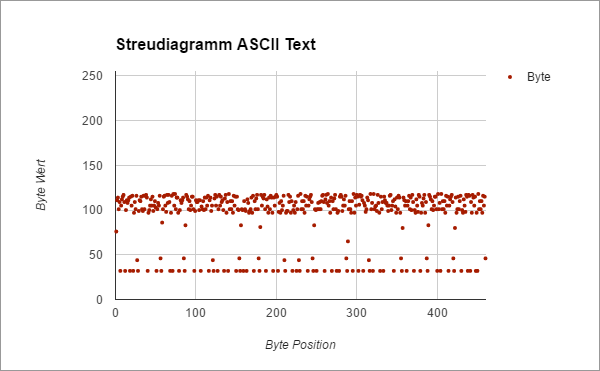
\includegraphics[scale=1]{images/L-whitening-clear.png}
		\caption{Hier deutlich zu erkennen die verwendeten ASCII Zeichen.}
		\label{fig:L: Whitening Clear}
	\end{figure}

	\begin{figure}[H]
		\centering
		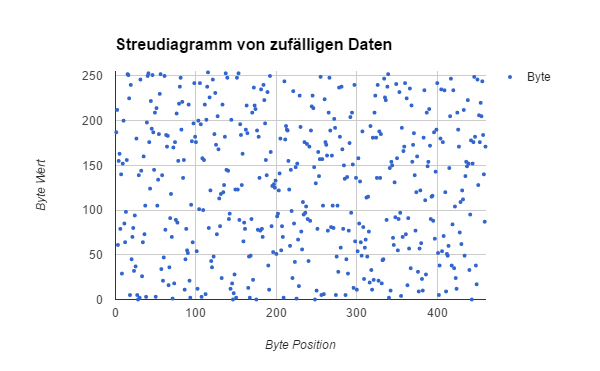
\includegraphics[scale=1]{images/L-whitening-random.png}
		\caption{In diesen zuf�lligen Daten kann kein Muster erkannt werden.}
		\label{fig:L: Whitening Random}
	\end{figure}
	
	\ltodo{H�here Aufl�sung f�r Whitening Diagramme https://docs.google.com/spreadsheets/d/1xDMWNJa9r2ggmzPAmDgE8qYJ5hk-8Hh9ZFuKrGrx7Gw}
	
	
	
	
     
	
	\subsubsection {Pseudozufallsgenerator mit bitweiser Verkn�pfung}
	
	Bei Verfahren welche auf Pseudozufallsgeneratoren bauen ist die gr��te St�rke auch gleich die gr��te Schw�che: ''Sie sind vorhersehbar''. Sie Sch�tzen zwar das Steganogramm vor unwissenden Dritten, wie so oft aber nicht wenn jemand gezielt danach sucht. Ihre sehr beschr�nkte Anzahl an Seeds und die Reproduzierbarkeit f�hren dazu das ein Angreifer sehr einfach auf die g�ngigsten Generatoren testen kann. 
	\\
	Das hier zur Anwendung kommende Prinzip ''Security through obscurity'' war bereits zu Beginn des 20. Jahrhunderts bekannt und auch als nicht sicher eingestuft. Das bekannteste Beispiel f�r Security through obscurity ist einen nicht standardisierten Port f�r eine Webanwendung zu verwenden. Dies Sch�tzt zwar vor automatisierten Bots, ein gezielter Angriff hebelt diesen ''Sicherheitsmechanismus'' innerhalb von Minuten aus. Genau so ist es mit schwachen Whitening Verfahren welche auf Obskurit�t setzen.
	\\
	In dem nachfolgenden Beispiel wird als Whitening der Datenstrom mit Hilfe der XOR-Operation mit einem Pseudozufallszahlengeneratoren Datenstrom verkn�pft. Zum Einsatz kommt hier ein Kongruenzgenerator wie er auch in der Standard Java Klasse java.lang.Random verwendet wird.  
	
	\begin{figure}[H]
	\begin{tabular}{|l|l|c|c|c|c|c|c|}
		\hline 
		& Byte 1 & Byte 2 & Byte 3 & Byte 4 & Byte 5 & Byte 6 \\ 
		\hline 
		Inhalt  & L & o & r & e & m &   \\ 
		\hline 
		Datenstrom & 76 & 111 & 114 & 101 & 109 & 32 \\ 
		\hline 
		Random (Seed=0) & 187 & 212 & 61 & 155 & 163 & 79 \\ 
		\hline 
		Datenstrom XOR Random & 247 & 187 & 79 & 254 & 206 & 111 \\ 
		\hline 
	\end{tabular} 	
    \caption{Wenn der Inhalt wieder hergestellt werden soll muss nur von unten nach oben alles wieder R�ckg�ngig gemacht werden.}
	\label{fig:L: Whitening Random Tabelle}
\end{figure}
	
	
	\begin{figure}[H]
		\centering
		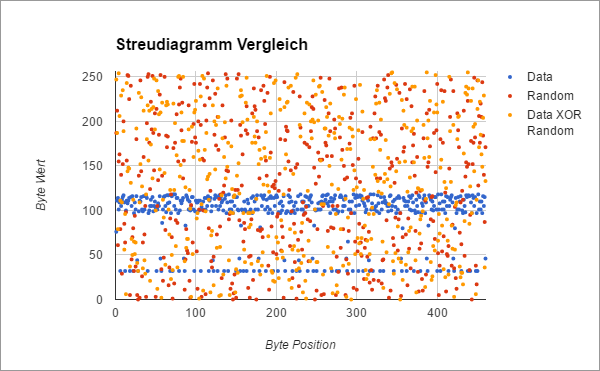
\includegraphics[scale=1]{images/L-whitening-vergleich.png}
		\caption{In diesem Vergleich ist gut zu sehen das nach Anwendung von diesem Verfahren der Datenstrom nicht mehr von zuf�lligen Werten unterscheidbar ist.}
		\label{fig:L: Whitening Random Vergleich}
	\end{figure}
	
	\subsubsection {AES-256 Verschl�sselung mit Key}
	
	Es kann auch die Eigenschaft von Verschl�sselung genutzt werden, Daten derart zu verarbeiten dass sie nicht mehr von zuf�lligen Werten unterscheidbar ist. In dem nachfolgenden Beispiel wird die zurzeit als sicher geltende AES-256 Verschl�sselung verwendet. 
	
	Folgende Java Funktion wurde f�r die Verschl�sselung des Plaintext verwendet:
	\lstinputlisting[firstline=30,lastline=42,caption={AESVerfahren.java},label={fig:L: AES Java}]{sources/AESVerfahren.java}
	
	Wenn man die daraus resultierenden Daten auswertet, l�sst sich wieder der gew�nschte Whitening-Effekt beobachten. 
	\begin{figure}[H]
		\centering
		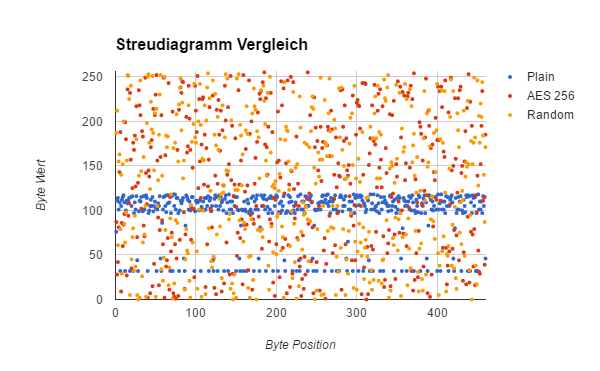
\includegraphics[scale=1]{images/L-whitening-aes.png}
		\caption{Vergleich zwischen AES verschl�sselten Daten und zuf�lligen Werten.}
		\label{fig:L: Whitening AES}
	\end{figure}

	
	\subsection{Fehlerkorrekturverfahren}
	
	Moderne Verfahren sind sehr anf�llig auf verlustbehaftete Komprimierung. Dadurch das sie meistens darauf basieren einzelne Bits zu ver�ndern, passiert es auch sehr schnell das die erneute Manipulation des Tr�germaterials zum Verlust der versteckten Daten f�hrt. In dem folgenden Abschnitt werden Techniken vorgestellt um diesen Informationsverlust zu verhindern oder wenigstens zu entdecken. Des weiteren werden mehrere Verfahren nach Robustheit verglichen.
	
	\subsubsection{Redundante Datenspeicherung}
	
	Eine M�glichkeit ist es die Daten mehrfach abzuspeichern. Das bietet Schutz vor Manipulation von einzelnen Teilen des Bild. Zum Beispiel das Wegschneiden von R�ndern, das Entfernen von Gesichtern, Wasserzeichen oder einfach Bild �ber- und Unterschriften welche erst sp�ter zu dem Bild hinzugef�gt werden.  
	
	Keine Verbesserung der Robustheit findet jedoch bei Komprimierung des Tr�germaterial statt, denn hier werden alle Teile geringf�gig ver�ndert was bereits ausreicht um einen kompletten Informationsverlust zu verursachen. 
	
	Auch wenn das Tr�germaterial vergr��ert/verkleinert wird Hilft redundante Speicherung meist nicht. Bei Skalierung von Bildern werden immer Filtering Methoden eingesetzt werden. Diese kombinieren oft mehrere Pixel zu einem einzelnen und wenden dabei zahlreiche Operationen an. Dadurch geht fast immer s�mtliche steganographisch versteckte Information verloren. 
	
	\subsubsection{Parit�tsbit}
	
	Die Parit�t einer Zahl beschreibt ob eine Zahl durch zwei Teilbar ist. Das Parit�tsbit wird zur �berpr�fung auf �bertragungsfehler verwendet indem es nach einer festgelegten Anzahl an �bertragenen Bits mitgesendet wird. Es werden die gesetzten Bits des zu �berpr�fenden Bereich gez�hlt. Ist dieser Wert nun eine gerade/ungerade Zahl wird das Parit�tsbit entsprechend gesetzt.

	Wenn im Laufe der �bertragung ein einzelnes Bit umgedreht wird kann dies durch das Parit�tsbit entdeckt werden. Der Fehler selbst kann dadurch aber nicht ausgebessert werden, da nicht bekannt ist wo er in der Bitfolge aufgetreten ist. Au�erdem kann nur eine ungerade Anzahl an Fehlern festgestellt werden. Eine Weiterentwicklung diese Verfahren stellt der unten vorgestellte Hamming-Code dar.
	
	\subsubsection{Zyklische Redundanzpr�fung (\zb CRC-32)}
	
	Die zyklische Redundanzpr�fung basiert auf Polynomdivison. Es wird ein CRC-Polynom gew�hlt  dessen Koeffizienten entweder 1 oder 0 sind. So entspricht etwa die Bitfolge 110101 dem Polynom $ x^{5} + x^{4} + x^{2} + 1$. 
	Die zu pr�fende Bitfolge wird nun mit einem Padding aus $n$ Nullen versehen, wobei $n$ dem Grad es Polynom entspricht. Das Ergebnis wird durch das CRC-Polynom dividiert, der Rest der Division an die Urspr�ngliche Bitfolge ohne Padding angeh�ngt und das ganze dann �bertragen. Dabei muss beachtet werden das bei der Division ausschlie�lich der XOR-Operator verwendet wird.
	Auf der Empf�ngerseite wird die gesamte �bertragene Bitfolge erneut durch das CRC-Polynom dividiert. Betr�gt der Rest Null dann ist entweder kein Fehler aufgetreten oder ein sehr unwahrscheinlicher. 
	Mit diesem Verfahren k�nnen nicht nur Fehler entdeckt, sondern im besten Fall sogar ausgebessert werden.
	
	

	
	Viele Dateiformate besitzen eine interne Angabe �ber wie lang die Datei sein sollte. Dies kann ausgen�tzt werden indem man eine Payload am Ende der Datei anf�gt. Programme welche die Tr�gerdatei lesen wollen ignorieren den zus�tzlich angeh�ngten Teil. Die versteckte Datei kann schnell und einfach wieder aus der Tr�gerdatei extrahiert werden. \\
	
	Zu beachten ist hier vor allem das man eine geeignete Tr�gerdatei w�hlt. Denn bei einer Datei welche sich oft in der L�nge �ndert kann es passieren das sein Versteckter angeh�ngter Teil einfach �berschrieben wird. Au�erdem sollte darauf geachtet werden dass die Datei eine fix definierte L�nge besitzt. Eine Beispiel f�r geeignete Dateiformate sind Bild- und Videoformate, sofern man sie nicht noch weiter bearbeiten will. Diese besitzen eine im Header der Datei angegebene L�nge und haben auch eine relativ gro�e Gr��e, wodurch kleinere angeh�ngte Dateien im Speicherplatzverbrauch nicht so stark auffallen. 
	
	
	\begin{figure}[H]
		\centering
		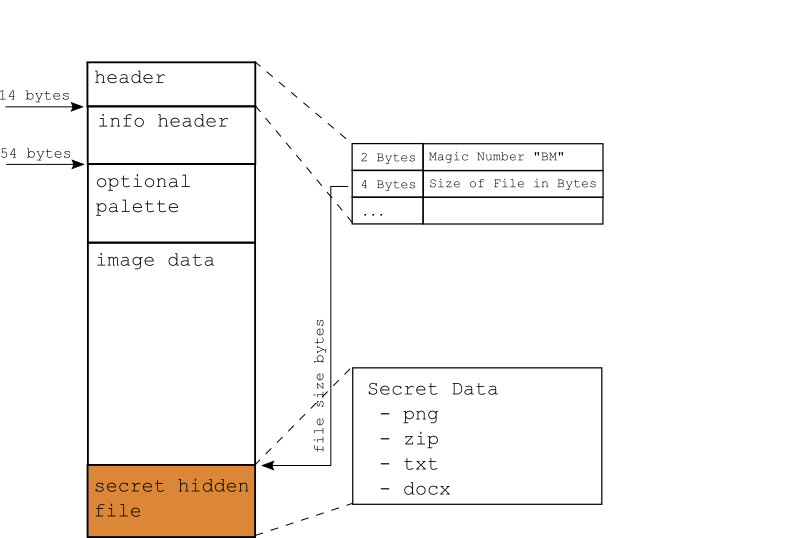
\includegraphics[scale=0.8]{images/L-bmp.png}
		\caption{Beispiel f�r das Verstecken einer Datei am Ende einer Bitmap}
		\label{fig:L: Datei in Bitmap}
	\end{figure}
	% http://paulbourke.net/dataformats/bmp/
	


	
	
	
	
	sub
	\section{Modifikation von Bilddateien} \ltodo{Die ganze Sache gibt es auch in der klassischen wo es darum geht z.B. in der L�nge der Gartenzaunbretter Informationen zu verstecken}
	
	Bilder auf einem Computer sind nichts anderes als Matrizen welche Farbeinformationen f�r die einzelnen Pixel des Bildes beinhalten. Es gibt zahlreiche Verfahren in diesen Daten zu verstecken. Im den folgenden Kapitel werden einige dieser Verfahren vorgestellt. Dadurch dass alle Daten im Computer in Bin�rform als Zahl gespeichert sind, ist es vollkommen egal welche Datei als Payload eingebettet wird. 
	
	Aus diesem Grund wird in den Beispielen die Kodierung aus \ref{L: Kodierung Payload} f�r die Payload verwendet.
	\begin{table}[]
		\centering
		\caption{Kodierungstabelle der Payload}
		\label{L: Kodierung Payload}
		\begin{tabular}{|lll|lll|lll|lll|}
			\hline
			\textbf{Zeichen} & \textbf{DEC} & \textbf{BIN} & \textbf{Zeichen} & \textbf{DEC} & \textbf{BIN} & \textbf{Zeichen} & \textbf{DEC} & \textbf{BIN} & \textbf{Zeichen} & \textbf{DEC} & \textbf{BIN} \\ \hline
			A                & 0            & 000000        & I                & 8            & 001000        & Q                & 16           & 010000        & Y                & 24           & 011000        \\
			B                & 1            & 000001        & J                & 9            & 001001        & R                & 17           & 010001        & Z                & 25           & 011001        \\
			C                & 2            & 000010        & K                & 10           & 001010        & S                & 18           & 010010        & Leerzeichen      & 26           & 011010        \\
			D                & 3            & 000011        & L                & 11           & 001011        & T                & 19           & 010011        & .                & 27           & 011011        \\
			E                & 4            & 000100        & M                & 12           & 001100        & U                & 20           & 010100        & ,                & 28           & 011100        \\
			F                & 5            & 000101        & N                & 13           & 001101        & V                & 21           & 010101        & ?                & 29           & 011101        \\
			G                & 6            & 000110        & O                & 14           & 001110        & W                & 22           & 010110        & !                & 30           & 011110        \\
			H                & 7            & 000111        & P                & 15           & 001111        & X                & 23           & 010111        & ''               & 31           & 011111        \\
			\hline
		\end{tabular}
	\end{table}
%	\begin{table}[]
%		\centering
%		\caption{Kodierungstabelle der Payload}
%		\label{L: Kodierung Payload}
%		\begin{tabular}{|lll|lll|lll|lll|}
%			\hline
%			\textbf{Zeichen} & \textbf{DEC} & \textbf{BIN} & \textbf{Zeichen} & \textbf{DEC} & \textbf{BIN} & \textbf{Zeichen} & \textbf{DEC} & \textbf{BIN} & \textbf{Zeichen} & \textbf{DEC} & \textbf{BIN} \\ \hline
%			A                & 32            & 100000        & I                & 40           & 101000        & Q                & 48           & 110000        & Y                & 56           & 111000        \\
%			B                & 33            & 100001        & J                & 41           & 101001        & R                & 49           & 110001        & Z                & 57           & 111001        \\
%			C                & 34            & 100010        & K                & 42           & 101010        & S                & 50           & 110010        & Zeilenumbruch    & 58           & 111010        \\
%			D                & 35            & 100011        & L                & 43           & 101011        & T                & 51           & 110011        & >                & 59           & 111011        \\
%			E                & 36            & 100100        & M                & 44           & 101100        & U                & 52           & 110100        & <                & 60           & 111100        \\
%			F                & 37            & 100101        & N                & 45           & 101101        & V                & 53           & 110101        & (                & 61           & 111101        \\
%			G                & 38            & 100110        & O                & 46           & 101110        & W                & 54           & 110110        & )                & 62           & 111110        \\
%			H                & 39            & 100111        & P                & 47           & 101111        & X                & 55           & 110111        & End of Message   & 63           & 111111        \\
%			\hline
%		\end{tabular}
%	\end{table}
	
	
	\subsection{Least Significant Bit Verfahren}
	
	Das Least Significant Bit (LSB) Verfahren n�tzt die Tatsache aus, dass der Farbraum einer modernen Bilddatei sehr gro� ist\footnote{Bei den meisten Formaten 24-Bit, wodurch 16,777,216 Farben dargestellt werden k�nnen}. Dadurch ist es f�r das menschliche Auge sehr schwierig, eng beieinander liegende Farbt�ne zu unterscheiden. Computerprogramme k�nnen nun gezielt einzelne Farben manipulieren um Informationen in den Pixel des Bildes zu kodieren. 
	
	Bei einem 24-Bit RGB Bild besteht jeder Farbkanal aus 8 Bit. Um die Nachricht zu kodieren wird das LSB von einem oder mehreren der Farbkan�le des Pixel auf den jeweiligen Wert aus der kodierten Nachricht gesetzt. Da das LSB nur einen wertm��igen Unterschied von +/-1 ausmacht wenn es ver�ndert wird, f�llt diese �nderung kaum auf. Wenn wir bei einem Pixel einen der Farbkan�le bearbeiten ver�ndern wir den Farbwert des Kanal um $\frac{1}{256} = 0.39\% $. Der Farbwert des Pixel �ndert sich sogar nur um $ \frac{1}{16777216} = 0.00000596\% $. Es ist so gut wie unm�glich mit dem freien Auge hier noch einen Unterschied zu erkennen.
	
	Ein gro�e Rolle spielt wie viel Tr�germaterial zur Verf�gung steht und wie viele Daten darin eingebettet werden. Je nachdem kann man die einzelnen Bits weiter verteilen oder muss sogar mehrere Bits auf ein Pixel. 
	Es ist auch durchaus sinnvoll diverse Pr�fsummen in die eingebetteten Daten einzubauen um sicher zu stellen das die extrahierten Daten auch keine Fehler enthalten. Wenn genug Platz zur Verf�gung steht ist es auch m�glich die Daten redundant zu speichern.
	
	\ltodo{Tabelle mit Vergleich wie viele Bit Farbe / wie viele Bit Daten und wie viel Prozent das ausmacht + Bildbeispiele f�r den Farbunterschied den das ausmacht}
	
	\begin{figure}[H]
		\centering
		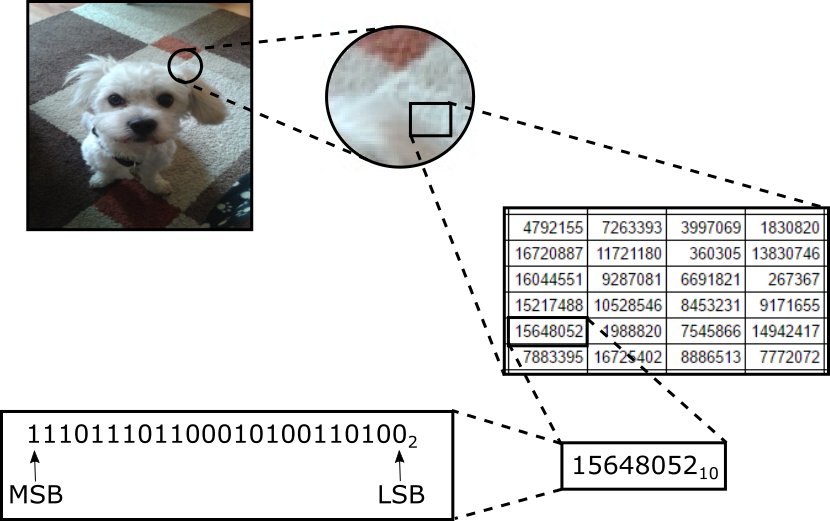
\includegraphics[scale=0.7]{images/L-lsb-entwurf.png}
		\caption{LSB Verfahren Erkl�rung}
		\label{fig:L: LSB in Bitmap}
	\end{figure}
	
	In dem Beispiel aus \ref{fig:L: LSB Tabelle} wurde eine Datendichte von einem Zeichen pro Pixel gew�hlt. Bei einem Bild mit 2  Megapixel lassen sich bis zu 2 Millionen Zeichen abspeichern. Das Buch ''Sch�ne neue Welt'' von Aldous Huxley hat rund 430.000 Zeichen, geht sich also bereits vier Mal in einem doch recht kleinen Bild aus. Das setzt aber Voraus das die in \ref{L: Kodierung Payload} angef�hrte Kodierungstabelle verwendet wird. Diese unterst�tzt aber weder Kleinbuchstaben noch Zeilenumbr�che, Umlaute oder Zahlen. Das Buch w�re durchaus noch lesbar, aber eben doch recht umst�ndlich. In der ASCII Kodierung hat das Buch eine Gr��e von 449.414 Bytes, also 3.595.312 Bits. Bei einer Datendichte von 6 Bit / Pixel geht sich das Buch dennoch in einem 2 Megapixel gro�en Bild aus.
	
	\begin{figure}[H]
		\centering
		\begin{tabular}{|c|c|c|c|c|c|c|c|}
			\hline 
			Pixel Nummer & 1 & 2 & 3 & 4 & 5 & 6 & 7 \\ 
			\hline 
			Nachricht & T & R & E & F & F & P & U \\ 
			\hline 
			Dec & 19 & 17 & 4 & 4 & 5 & 15 & 20 \\ 
			\hline 
			Bin�r & 10011 & 10001 & 00100 & 00100 & 00101 & 01111 & 10100 \\ 
			\hline 
			Roter Farbwert & RRRR RR10 & RRRR RR10 & RRRR RR00 & RRRR RR00 & RRRR RR00 & RRRR RR01 & RRRR RR10 \\ 
			\hline 
			Gr�ner Farbwert & GGGG GG01 & GGGG GG00 & GGGG GG10 & GGGG GG10 & GGGG GG10 & GGGG GG11 & GGGG GG10 \\ 
			\hline 
			Blauer Farbwert & BBBB BBB1 & BBBB BBB1 & BBBB BBB0 & BBBB BBB0 & BBBB BBB1 & BBBB BBB1 & BBBB BBB0 \\ 
			\hline 
		\end{tabular} 
		\caption{Beispiel f�r Kodierung von einem Zeichen pro Pixel.}
		\label{fig:L: LSB Tabelle}
	\end{figure}
	
	In dem in \ref{fig:L: LSB Earth} gezeigtem Beispiel wurde das Buch ''Sch�ne neue Welt'' in ein Bild der Erde integriert. Verwendet wurde das in \ref{fig:L: LSB Java} gezeigte Java-Programm. Die kurze L�nge des Programm zeigt das dieses Verfahren sehr einfach zu implementieren ist. Man kann durchaus, egal wo man sich gerade befindet, mit Hilfe eines Computers ein Programm schreiben und geheime Nachrichten versenden. Durch den  zus�tzlichen Einsatz von Whitening kann also von �berall aus eine steganografisch sichere Daten�bermittlung stattfinden, ohne vora. 
	
	\begin{figure}[H]
		\centering
		\includegraphics[scale=0.3]{images/L-schoene-neue-earth.png}
		\caption{In diesem Bild wurde ein ganzes Buch versteckt, und es ist trotzdem nicht zu erkennen.}
		\label{fig:L: LSB Earth}
	\end{figure}

	\lstinputlisting[caption={LSBVerfahren.java},label={fig:L: LSB Java}]{sources/LSBVerfahren.java}

	
	Wenn die einzubettenden Daten nicht den gesamten Verf�gbaren ''Speicherplatz'' innerhalb des Steganogramm verwenden, sollte unbedingt ein Padding aus zuf�lligen Daten hinzugef�gt werden. Sonst k�nnen sich deutliche Unterschiede in dem Aussehen des Bild ergeben wenn es gro�e, einfarbige Fl�chen besitzt, wie in \ref{fig:L: LSB No Padding} deutlich zu erkennen ist.
	
	\begin{figure}[H]
		\centering
		
\includegraphics[scale=0.3]{images/L-lsb-sichtbare-einbettung.png}
		\caption{Auf der linken Seite befinden sich eingebettete Daten, auf der rechten Seite nicht.}
		\label{fig:L: LSB No Padding}
	\end{figure}
	
	
	Die resultierende Datei ist deutlich gr��er als die Originale. Das liegt daran dass durch das einbetten der Daten gro�e einfarbige Fl�chen minimal ver�ndert wurden, wodurch sie sich nicht mehr so gut komprimieren lassen wie zuvor.
	
	
	\subsubsection{Varianten des Least Significant Bit Verfahren}
	
	\subsection{Barcode Verfahren}
	
	Das Barcodeverfahren ist ein selbst erfundenes Verfahren welches einen Barcode in einem Bild versteckt. Dies geschieht indem das Bild zuerst in ein 8-Bit Graustufenbild konvertiert und anschlie�end das Histogramm des Bildes generiert wird. 
	
	Ein Histogram ist eine grafische Abbildung der Anzahl einzelner Farbwerte. In das  \ref{fig:L: Barcode Example}  wurde das Bild zuerst in ein 8-BGraustufenbild umgewandelt, die entstehenden 256 verschiedenen Werte gez�hlt und grafisch Dargestellt. 
	
	Wenn man nun das Bild gezielt so bearbeitet das bestimmte Farbwerte nicht mehr vorkommen, dann ergeben sich dadurch auch im Histogramm entsprechende Spalten. Mit dieser Hilfe kann nun jedes beliebiges eindimensionale Barcodeformat eingebettet werden.
	
		
	
	\begin{figure}[H]
		\centering
		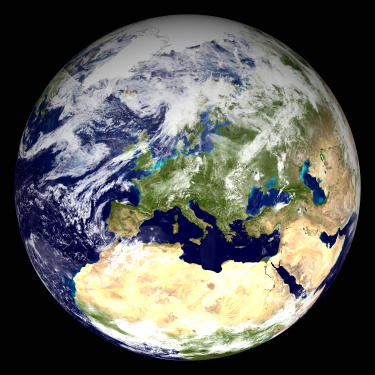
\includegraphics[scale=0.02]{images/L-earth.png}
		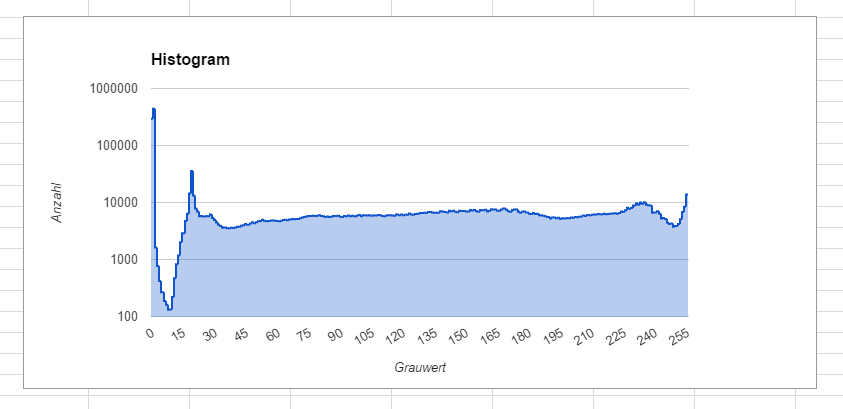
\includegraphics[scale=0.3]{images/L-barcode-example.png}
		\caption{}
		\label{fig:L: Barcode Example}
	\end{figure}
	
	
	Damit g�ngige Barcodescanner jedoch den Barcode wahrnehmen k�nnen muss das Histogramm grafisch gewisse Anforderungen erf�llen. Die meisten vorhandenen Histogramm Generatoren stellen das Resultat in einer sch�nen ansprechenden Form dar, \zb der Graph gegl�ttet und in Farbe. Barcodescanner brauchen aber schwarze Striche welche deutlich voneinander unterscheidbar sind. Deshalb muss ein spezieller Barcodegenerator verwendet werden.
	
	 Ein Beispiel f�r einen solchen Generator findet sich in \ref{fig:L: HistogramViewer}. Dieses Programm generiert dann f�r Barcodescanner verwendbare Histogramme, wie in \ref{fig:L: Barcode Histogram Example} gezeigt wird. In diesem Beispiel wurde das g�ngige Barcodeformat CODE\_128 verwendet und der Text ''Simon Lehner-D.'' damit kodiert.
	
	\begin{figure}[H]
		\centering
		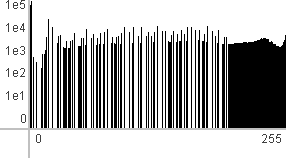
\includegraphics[scale=1.5]{images/L-histogram-viewer-output.png}
		\caption{fig:L: Barcode Histogram Example}
		\label{fig:L: Barcode Histogram Example}
	\end{figure}
	
	\ltodo {Einfach nur den link zum git repo reintun?}
	\lstinputlisting[caption={HistogramViewer.java},label={fig:L: HistogramViewer}]{sources/HistogramViewer.java}
	
	
	
	
	
	
	
	
	
	
	\subsection{Stereoskopische Verfahren}
	
	Die Stereoskopie beschreibt Methoden um auf Bildern den Eindruck zu machen, dass diese drei Dimensional sind, obwohl physikalisch gar keine Tiefe vorhanden ist. Sie macht sich dabei zur Hilfe, dass das Gehirn eigentlich nur zwei 2D Aufnahmen der Umgebung bekommt und diese dann erst als 3D Gebilde interpretiert. 
	
	Um im Gehirn den Eindruck von r�umlicher Tiefe zu erzeugen m�ssen beide Augen die selbe Szene aus zwei verschiedenen Blickwinkel zu sehen bekommen. Dies funktioniert normalerweise dadurch das beide Augen in einem Abstand von ungef�hr 15cm voneinander entfernt sind. Wenn nun aber beide Blickwinkel mit einer Kamera aufgenommen und nebeneinander gelegt wurden muss man dem Gehirn etwas nachhelfen. Mit der richtigen Blicktechnik, \zb durch Schielen, k�nnen die beiden Teilbilder wieder �bereinandergelegt werden und der gew�nschte tiefen Effekt tritt auf.
	
	\begin{figure}[H]
		\centering
		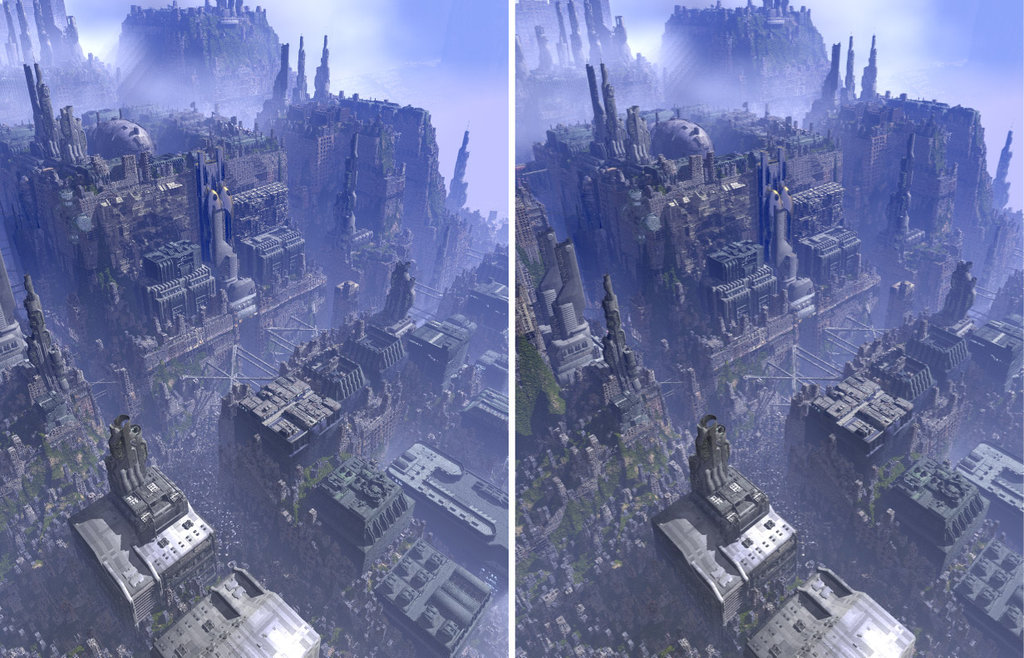
\includegraphics[scale=1.5]{images/L-stereogram-example.jpg}
		\caption{fig:L: Stereogramm Example}
		\label{Beispiel fr ein Stereogramm}
	\end{figure}
	\ltodo{Quelle raus suchen oder eigenes Bild aufnehmen}
	
	Es gibt verschiedene Techniken um Stereogramme zu erstellen, die sich vor allem durch die Wahl des Tr�germaterial unterscheiden
	
	\begin{itemize}
		\item Classic stereogram
		
		Das klassiche Stereogramm aus 2 Bildern, welche mit der richtigen Blicktechnik oder einem Stereoskop dreidimensional gesehen werden k�nnen. 
		
		
		\item Single image stereogram (SIS) 
		
		Einzelbildstereogramme, auch oft Autostereogramm genannt, verwenden wie der Name schon sagt nur ein einzelnes Tr�gerbild um die Formen zu beinhalten. Dazu ben�tigen sie ein sich wiederhohlendes Muster in welches mit Hilfe eines Programm und einer Depthmap die Formen hinzugef�gt werden.
		
		Grunds�tzlich kann jede der hier genannten Techniken auch Autostereogramme erzeugen.
		
		\item Random dot stereogram (RDS)
		
		Bei diesem werden Bilder bestehend aus zuf�lligen Punkten verwendet um dreidimensionale Formen darzustellen. Dadurch ist es oft auf den ersten Blick nicht gleich ersichtlich, dass es sich hier um ein Stereogramm handelt.
		
		\item Text stereogram
		
		Als Tr�germaterial wird ausschlie�lich Text verwendet. Ein Beispiel daf�r ist unter \ref{fig:L: Stereogramm Example ASCII} zu sehen.
		
		\item Map textured stereogram 
		
		Diese Technik ist sehr �hnlich wie RDS, nur das hier Texturen wie sie in etwa Videospielen vorkommen verwendet werden. Diese haben die Eigenschaft beliebig oft wiederholt werden zu k�nnen, ohne das sich Kanten im Bild ergeben. Dadurch l�sst sich sehr gut ein Stereogramm daraus erzeugen.
		
		Die bekannte Buchserie ''Magic Eye'' beinhaltet vor allem solche Stereogramme, weil die Blicktechnik hier einfacher anzuwenden ist als \zb bei Text Stereogrammen.
		
		\item Wallpaper stereogram / object array stereogram
		
		Bei einem Objekt Array Stereogramm wird ein und dasselbe Bild mehrere male wiederholt. Dabei werden aber die Abst�nde von einzelnen Elementen des Bild unterschiedlich gew�hlt um den gew�nschten 3D Effekt zu erzielen.
		
		
	\end{itemize}
	
	
	
	\begin{figure}[H]
		\centering
		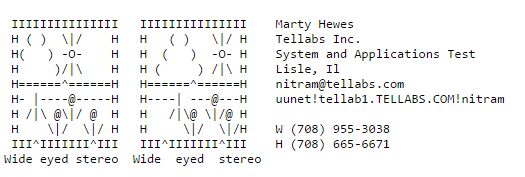
\includegraphics[scale=1.0]{images/L-stereogram-ascii.png}
		\caption{fig:L: Stereogramm Example ASCII}
		\label{Beispiel fr ein Text Stereogramm}
	\end{figure}
	\ltodo{Quelle: https://web.archive.org/web/20080517013244/archive.museophile.org/3d/ascii-3d.html}
	
	
	
	\begin{figure}[H]
		\centering
		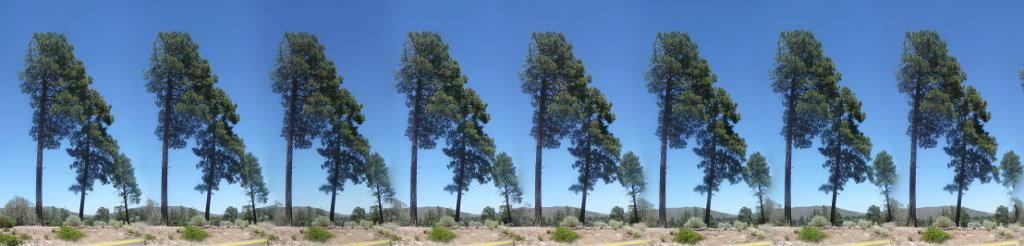
\includegraphics[scale=0.40]{images/L-stereogram-tree.jpg}
		\caption{fig:L: Stereogramm Example Object Array}
		\label{Beispiel fr ein Objekt-Array Stereogramm}
	\end{figure}
	\ltodo{Quelle: http://www.pakin.org/~scott/stereograms/}
	
	Aus diesen Techniken ergeben sich nun einige praktische Anwendungsm�glichkeiten, welche im folgenden genauer bearbeitet werden. Des weiteren werden Hilfmittel gezeigt mit deren Hilfe man Stereogramme automatisch entdecken und Entschl�sseln darstellen kann.
	
	
	\subsubsection{Erzeugen von Stereogrammen mithilfe einer Depth Map}
	
	Zuerst ben�tigt man sowohl ein gutes Muster als Grundlage als auch eine sogenannte Depth Map. Depth-Maps sind im Grunde einfach Schwarz-Wei� Bilder bei denen der Wei�wert jedes Pixels die Tiefe/H�he der jeweiligen Position angibt.
	Beide Teile gibt es zahlreich im Internet. Bei Bedarf k�nnen Depth Maps auch mit einer geeigneten 3D-Grafiksuite wie etwa Blender erzeugt werden. Aber auch einfache Bildbearbeitungsprogramme sind gut dazu geeignet vor allem Text als Depth Map abzuspeichern.
	
	Dabei gilt vor allem der Grundsatz: Je einfacher das dargestellte Objekt in der Depth Map, desto einfacher ist es auch das Stereogramm ohne technischer Hilfsmittel dreidimensional sehen zu k�nnen.
	
	
	Um das Stereogramm nun zu erzeugen wird ein neues leeres Bild erzeugt mit der selben gr��e wie die Depth Map. Auf diesem Bild wird nun das gew�hlte Muster auf dem linken Rand hineinkopiert, so dass es von oben bis unten einen Streifen mit dem Muster bildet. Die Gr��e dieses Grundstreifen wird von nun an $N$ genannt gibt an um wie viel die Augen das Bild verschieben m�ssen um auf der Grundtiefe zu sein. 
	
	Die restlichen noch leeren Teile des Bildes werden nun erzeugt indem immer das Pixel auf der selben H�he um $N$ nach links verschoben kopiert wird. Um den gew�nschten Tiefeneffekt zu bekommen wird noch jeweils ein Offset hinzugef�gt das dem Wert der aktuellen Position auf der Depth Map entspricht.
	
	
	$$
	E(x,y)=
	\begin{cases}
	M(x,y), & \text{if } x < N \\
	E(x - N + (s * D(x,y)), & \text{else}
	\end{cases}
	$$

	\begin{itemize}
		\item \textbf{$E(x,y)$} das resultierende Stereogramm
		\item \textbf{$M(x,y)$} das Muster welches als Grundlage verwendet werden soll.
		\item \textbf{$D(x,y)$} die Depth Map $[0.0;1.0]$
		\item \textbf{$s$} ein Faktor der Angibt wie gro� der Tiefeneffekt sein soll $[0.0;N]$
	\end{itemize}

	\begin{figure}[H]
		\centering
		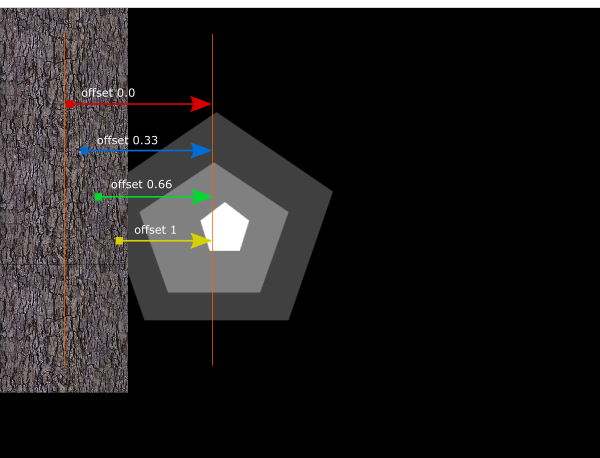
\includegraphics[scale=1]{images/L-stereogram-anleitung.png}
		\caption{Die Pixel werden je nach Depth Map vom linken Strich + Offset zu dem rechten Kopiert.}
		\label{fig:L: Stereogramm Anleitung}
	\end{figure}

	Wiederholt man diesen Vorgang �ber das gesamte Bild ergibt sich dann folgendes Stereogramm.
	\begin{figure}[H]
		\centering
		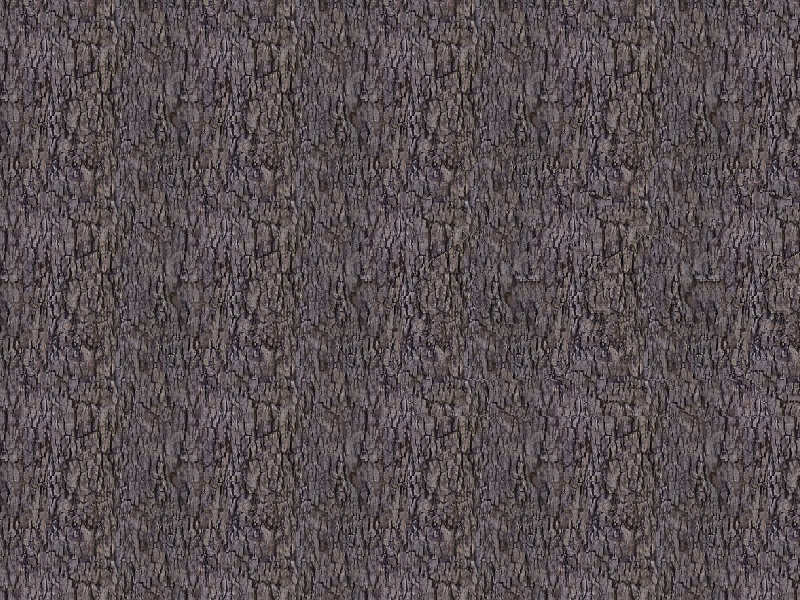
\includegraphics[scale=0.4]{images/L-stereogram-selber.png}
		\caption{Kaum zu erkennen sind die versteckten Formen.}
		\label{fig:L: Stereogramm Anleitung}
	\end{figure}
	
	Verwendet wurde daf�r dieses Java-Programm:
	\lstinputlisting[caption={StereogrammGenerator.java},label={fig:L: Stereogramm Generator in  Java}]{sources/StereogrammGenerator.java}
	
	
	
	\subsubsection{Steganographie mithilfe von Stereogrammen}
	
	Ein Autostereogramm ist eigentlich schon ein Steganogramm, da ja der eigentliche Inhalt auf den ersten Blick nicht ersichtlich ist. Wenn man ein Schwarz/Wei� Bild mit Text drauf als Depth Map verwendet ergibt das ein Stereogramm welches einen geheimen Text enth�lt. 
	
	
	\subsubsection{Grafisches Hilfsmittel zum Entschl�sseln von Stereogrammen}
	
	Wenn man nun keine Motivation oder nicht gen�gend Zeit hat die richtige Blicktechnik zu erlernen kann man auf technische Hilfsmittel zur�ckgreifen.
	
	Meistens reicht es aus einfach das Bild in einem geeigneten Bildbarbeitungsprogramm zu �ffnen und dort richtig zu bearbeiten: Es muss das gesamte Bild kopiert und wieder eingef�gt werden. Das eingef�gte Bild wird dann auf der selben H�he solange nach links und rechts verschoben bis man den gew�nschten Effekt erzielt. Dabei ist zu beachten, dass das Programm die Composite-Einstellungen ''Differenz'' unterst�tzt und diese auch verwendet wird. Das Wort Composite kommt aus dem Englischen und bedeutet so viel wie Zusammensetzung oder Gemisch. Im Sinne von Bildbearbeitung ist damit gemeint auf welche Art und Wei�e die Pixel miteinander verbunden werden sollen. F�r Stereogramme m�ssen die Pixel voneinander subtrahiert werden, es wird also die Differenz der Pixel ben�tigt. Daher auch die entsprechende Einstellung. 
	
	Wenn der Bedarf da ist, des �fteren Stereogramme zu Entschl�sseln, dann ist es oft Hilfreich ein kleines Programm daf�r zu verwenden. Es gibt zum Beispiel eine Implementierung eines solchen Programm unter \url{http://magiceye.ecksdee.co.uk/}. Diese verwendet jedoch Low-Level Javascript Array Operationen, wodurch die Anwendung bei sehr gro�en Dateien zu langsam und damit unbrauchbar ist.
	
	 Moderne Browser unterst�tzen f�r die Rendering Kontexte in Javascript die oben erw�hnten Composite-Operationen. Daher kann eine eigene kleine Funktion als Solver in nicht mehr als 5 Lines of Code geschrieben werden. Diese verwendet Hardwarebeschleunigung und ist somit selbst bei riesigen Dateien noch ausreichend schnell. Diese Funktion muss nur noch in eine kleine Oberfl�che verpackt werden und ist schon einsatzbereit.
	 
	 \lstinputlisting[caption={Einfacher Stereogramm Solver},label={fig:L: Stereogramm Solver}]{sources/StereogrammSolverShort.js}
	 \ltodo{Javascript wird nicht unterstuetzt}
	 
	 
	 \ltodo{Stereogramme mit verlaufenden 3D Bildern sind etwas komplizierter zum schoen darstellen, muss ich nur implementieren, hab da schon ne idee}
	
	\subsubsection{Automatische Erkennung von Stereogrammen}
	
	Es gibt noch kein Standardverfahren zur Erkennung ob es sich bei einem Bild um ein Stereogramm handelt. Deswegen wurde im Rahmen des Projekt Geocaching-Tools und f�r diese Diplomarbeit ein  eigenes entwickelt. 
	
	Wie bereits bei den grafischen Hilfsmittel zum Entschl�sseln von Stereogrammen gezeigt werden Stereogramme beim Verarbeiten eine Kopie des Bildes um ein gewisses Offset nach rechts verschoben und anschlie�end vom Bild subtrahiert. Die Herausforderung und das Ziel des Verfahren ist es also das richtige Offset, falls vorhanden, zu erkennen. 
	
	Dabei werden ganz �hnlich wie man es bei dem grafischen Hilfsmittel per Hand machen kann alle m�glichen Verschiebungen generiert. Zwei identische Farben voneinander Subtrahiert ergeben die Farbe schwarz. Es wird also nach einem Offset gesucht bei dem ein M�glichst gro�er Teil des Bildes Schwarz wird. Damit ist auch schon der gr��te Teil der Arbeit getan. Aus den prozentualen Schwarzanteilen vom Gesamtbild �ber die verschiedenen Verschiebungen ergibt sich f�r jedes Bild eine Datenserie. Diese muss nur noch Analysiert werden. 
	
	In \ref{fig:L: Stereogramm Erkennung Vergleich} sind vier Bilder mit dieser Technik analysiert worden. Dabei kann man gut erkennen dass sich ein Spike in der Datenreihe ergibt wenn das Bild ein Stereogramm ist. Das gr��te Problem bei der Sache sind Bilder welche im vor hinein bereits gr��ten Teil aus schwarz bestehen. Auch Signaturen von Bildern welche nur sehr wenige Farben beinhalten sind oft den Signaturen von Stereogrammen sehr �hnlich. Ein Beispiel daf�r sind Bilder mit viel wei�em Text auf schwarzem Hintergrund.
	
	\begin{figure}[H]
		\centering
		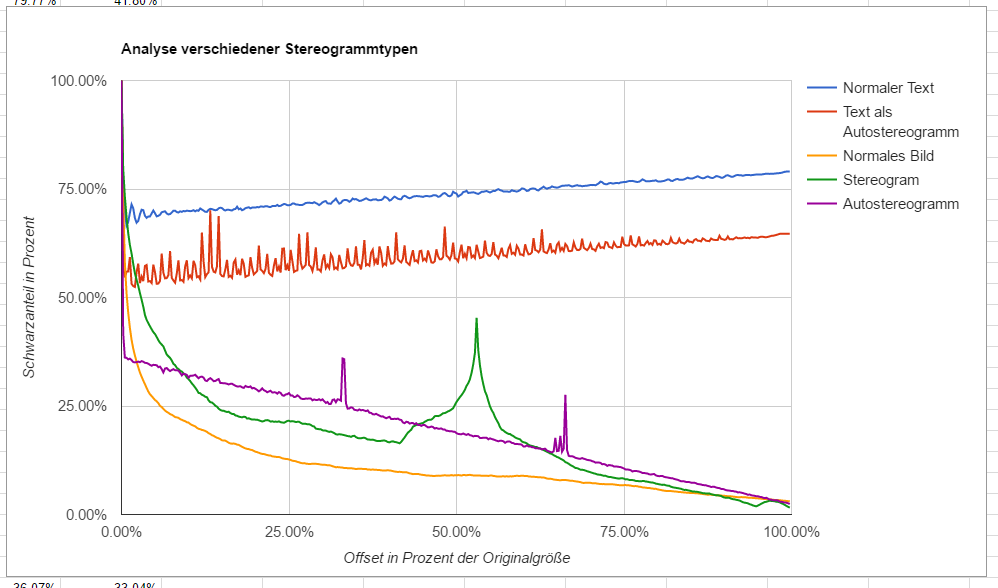
\includegraphics[scale=0.5]{images/L-stereogram-erkennung-vergleich.png}
		\caption{Bei dem Stereogramm kann ein Spike in der Datenreihe erkannt werden}
		\label{fig:L: Stereogramm Erkennung Vergleich}
	\end{figure}

	Stereogramme haben mit dieser Analyse immer einen Spike in der Datenreihe w�hrend normale Bilder einen eindeutigen Abw�rtstrend haben. Lediglich Texte sind schwer zu unterscheiden und einzuordnen. Eine M�glichkeit w�re nun eine k�nstliche Intelligenz darauf zu trainieren, diese Datenreihen zu analysieren. Die hier generierten Daten eignen sich sehr gut f�r ein solches Verfahren weil sie Aufgrund der prozentuellen Angaben eine fixe Gr��e besitzen. Daf�r wird jedoch sehr viel Rechenleistung ben�tigt, wodurch hier eine effizientere Methode gew�hlt wurde.
	
	Gesucht wird die gr��te Steigung zweier Punkte. Also $ d(j) - d(i) , i > j $ soll maximiert werden. Dazu wurde folgender sehr einfacher und schneller Algorithmus gew�hlt:
	
	\lstinputlisting[caption={Steigung},label={fig:L: Steigung Java}]{sources/Steigung.java}
	
	Das Problem was sich hier jedoch ergibt ist, dass wie in \ref{fig:L: Stereogramm Erkennung Vergleich} zu sehen ist, Texte eine recht hohes Ergebnis bei diesem Test erzielen, da sie einen steigenden Trend besitzen. Dies Ergibt sich aus dem hohen Schwarzanteil des Originalbild. Dadurch das bei der Berechnung auch der sich nicht mit dem verschobenen Bild �berschneidende Teil miteinbezogen wird, f�hrt das zu diesen sehr hohen Werten. 
	
	Wenn bei dem Algorithmus nur der Teil zur Berechnung herangezogen von dem das verschobenen Bild 
	subtrahiert wurde ver�ndern sich die Datenreihen deutlich: Die Spikes bei Stereogrammen vergr��ern sich um ein vielfaches und der generelle Trend wird flacher. 
	
	\begin{figure}[H]
		\centering
		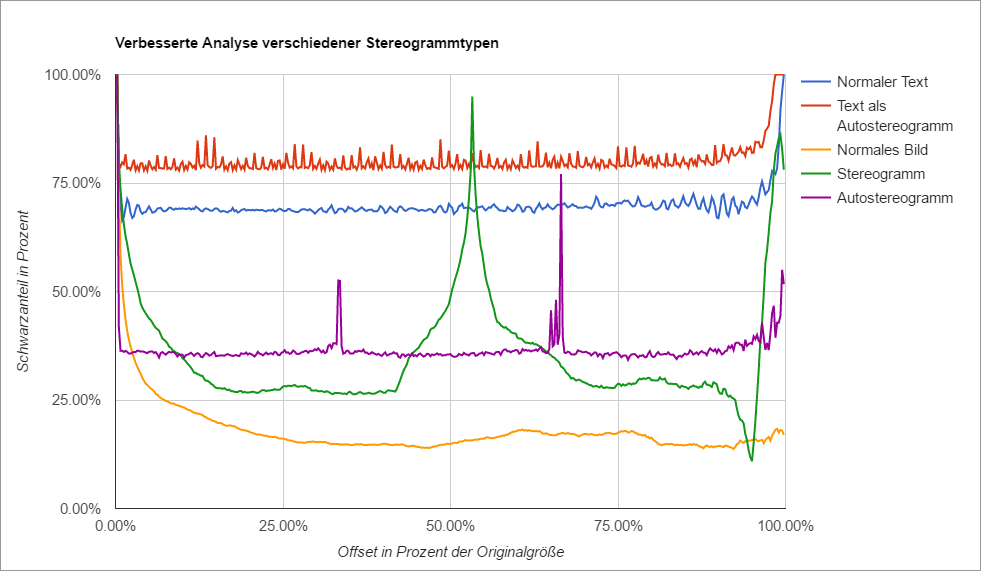
\includegraphics[scale=0.5]{images/L-stereogram-erkennung-vergleich-besser.png}
		\caption{Die verbesserte Variante erzielt deutlichere Ergebnisse}
		\label{fig:L: Stereogramm Erkennung Vergleich Verbessert}
	\end{figure}

	Es ist aber auch zu beobachten das im letzten Viertel die Werte sehr stark zu schwanken anfangen. Das liegt daran dass der beobachtete Bereich immer kleiner wird und dadurch sehr wenige kleine �berschneidungen einen sehr gro�en Effekt auf das Ergebnis haben. Um noch bessere Ergebnisse zu erzielen kann also das letzte Viertel der Datenreihe vernachl�ssigt werden, da es bei einem Offset von mehr als 75\% sehr unwahrscheinlich ist das es sich hier noch um ein Stereogramm handelt.
	
	In der folgenden Grafik werden die drei Versionen miteinander Verglichen.
	\begin{figure}[H]
		\centering
		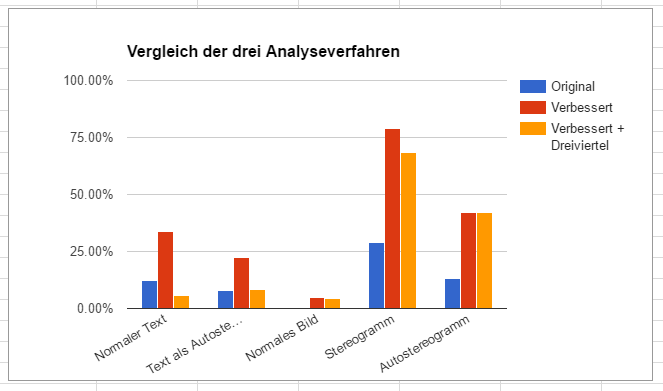
\includegraphics[scale=0.8]{images/L-stereogram-erkennung-vergleich-ergebnisse.png}
		\caption{Ein Wert von mehr als 25\% hei�t, dass es sich Wahrscheinlich um ein Stereogramm handelt.}
		\label{fig:L: Stereogramm Erkennung Vergleich Verbessert}
	\end{figure}
	
	
	Wie zu sehen ist erzielt das eben vorgestellte Verfahren bei vier von f�nf Testf�llen ein korrektes Ergebnis. Um eine 100\% korrekte Aussage treffen zu k�nnen werden kompliziertere Verfahren ben�tigt, wie die oben vorgeschlagene Verwendung von k�nstlicher Intelligenz.
	
	
	\subsubsection{Bildfehler erkennen}
	
	Jeder kennt diese Suche den Fehler Bilder aus Tageszeitungen. Diese bestehen aus zwei beinahe identischen Bildern. Bei einem der beiden wurden jedoch einzelne Details entfernt. Das ist �hnlich wie bei herk�mmlichen Stereogrammen, bei denen die einzelne Teile zwar nicht entfernt, sondern verschoben sind.
	
	
	Dadurch das diese beiden Anwendungen so �hnlich sind, kann man sehr gut Hilfsmittel aus der Stereographie anwenden um die Bildfehlerspiele zu l�sen. Wenn man die Blicktechniken von Stereogrammen auf diese Spiele anwendet, �berlappen die beiden Bilder derart, dass auf der selben Stelle der entfernte Teil sichtbar und unsichtbar ist. Deshalb wei� das Gehirn nicht welches der beiden Augen recht hat, weil das linke Auge zum Beispiel eine Schornstein sieht und das Rechte nicht. Diese Teile des Bildes schauen dann aus als w�rden sie Flimmern.
	
	Wenn ein automatisches Hilfsmittel auf ein derartiges Bildpaar angewendet wird, dann ergibt sich bei dem richtigen Offset ein schwarzes Bild auf dem nur die Fehler als Farbhaufen zu sehen sind. Im Sinne der Steganographie kann zum Beispiel der Sekundenteil einer Koordinate als Position auf einem Quadratischen Bild mit je 1000px Seitenl�nge markiert werden, indem dort der Bildfehler platziert wird.
	
	\ltodo{Finde ein Beispiel f�r ein solches Suchbildr�tsel und l�se es mit GC-Tools}
	
	
	
	\subsection{Grafische Verfahren}
	\ltodo{
		Gemeint sind hier Verfahren welche direkt grafische Elemente zu einem Bild hinzuf�gen.
		Zum Beispiel irgendwo im Bild einen Morsecode/Barcode/Blindenschrift indem zum Beispiel Grashalme hinzugef�gt werden.
		Vllt zu klassische Verfahren
	}
	
	\subsection{Odd-Pixel Verfahren}
	
	Das Wort ''Odd'' kommt aus dem Englischen und bedeutet seltsam oder merkw�rdig. Es handelt sich also um merkw�rdige Pixel. Damit ist zum Beispiel gemeint wenn in einem fast komplett dunklen Bild irgendwo ein einzelnes Pixel Wei�, Grasgr�n oder Rubinrot ist. So ein seltsames Pixel f�llt einem sofort auf: Das passt da einfach nicht rein. 
	
	Man kann sich das zu Nutze machen indem man dem Odd-Pixel eine ganz bestimme Position oder eine spezielle Farbe gibt. Ein Beispiel: Ein gr�nes Odd-Pixel bedeutet ja und ein rotes nein oder die Position gibt die Koordinaten f�r einen Treffpunkt an. 
	
	Wenn man ein solches Odd-Pixel verstecken will muss man aber beachten dass die Wahrnehmungsschwelle eines Menschen nicht unterschritten wird. Sonst f�hrt das unweigerlich dazu, dass niemand das Steganogramm entziffern kann. Jedoch ist es kaum beeinflussbar f�r wen das Pixel sichtbar ist, wessen Wahrnehmungsschwelle also ausreicht. 
	
	Eine gro�e Herausforderung stellt hier vor allem die automatische Erkennung eines solchen Odd-Pixel dar. Wei� man wonach man sucht macht es die ganze Sache schon einfacher. Wird zum Beispiel ein komplett wei�es Pixel gesucht, also mit den allen Werten der RGB-Skala auf 255, so muss das Programm nur eben dieses Pixel aufsp�ren. Es ist also das beste ein Programm zur Verf�gung zu stellen welches diese Aufgabe zwar nicht von alleine l�sen kann, jedoch einem Menschen bei der Arbeit unterst�tzt.
	
	Um das einfache Arbeiten zu erm�glichen sind folgende Funktionen n�tzlich:
	\begin{itemize}
		\item Eine Zoomfunktion
		\item Markieren von Stellen mit einem Stift/Radierer Werkzeug
		\item Filtern nach bestimmten Farben. �hnlich dem F�llwerkzeug bei Bildbearbeitungsprogrammen, nur als einstellbarer Filter welcher Bereiche verdunkelt welche nicht dem Kriterium entsprechen.
		\item Automatisches Markieren von gefundenen Stellen. Einzelne Pixel sind sehr schwer zu sehen, selbst wenn diese eingef�rbt wurden. Eine Art bunte Umrandung ist dabei sehr hilfreich. 
		\item Gruppieren von benachbarten Pixeln. Diese Pixelgruppen dann in einer ausw�hlbaren Liste darstellen um Position, Farbe und weitere Eigenschaften abrufen zu k�nnen.
	\end{itemize}
	
	Mithilfe diesen Funktionen sollte es nicht mehr allzu schwer sein Odd-Pixel zu finden.
	
	Erw�hnenswert ist hier eine einfache Technik mit deren Hilfe einzelne Pixel sowie Pixelgruppen umrandet werden k�nnen. Es handelt sich um einen Filter und zwei Pinsel Operationen welche nacheinander auf die Auswahlmaske angewendet werden. 
	
	Ein Pinsel wird auf das ganze Bild angewendet indem f�r jeden Punkt auf dem Bild �berpr�ft wird ob eine bestimmte Bedingung eintrifft und wenn ja wird ein Kreis in der angegebenen Gr��e mit einer bestimmten Farbe dort hin gezeichnet.
	
	Ein Filter bestehen aus einem sogenannten Kernel, ein zwei dimensionales Zahlenarray. Wie in \ref{fig:L: Odd Pixel Conv} dargestellt wird jeder Wert aus dem Kernel auf den Input mit einer festgelegten Operation verkn�pft und die Ergebnisse summiert. Wenn nicht genauer definiert ist die verwendete Operation die Multiplikation. Zahlreiche bekannten Filter und Effekte aus Bildbearbeitungsprogrammen k�nnen auf diese Weise implementiert werden. 
	
	\begin{figure}[H]
		\centering
		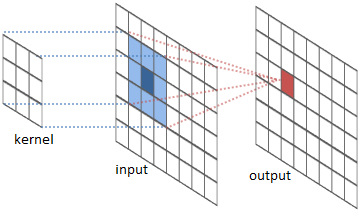
\includegraphics[scale=0.5]{images/L-odd-pixel-conv.png}
		\caption{Kernel wird auf den Input angewendet um den Output zu erzeugen.}
		\label{fig:L: Odd Pixel Conv}
	\end{figure}
	
	
	Einige Anwendungsbeispiele f�r Kernel sind:
	\begin{itemize}
		\item Laplacian Kantenerkennungs Kernel \\
		$
		K =\begin{bmatrix}
			-1 & -1 & -1 \\
			-1 & 8  & -1 \\
			-1 & -1 & -1
		\end{bmatrix}
		$		
		$
		K = \begin{bmatrix}
		0 &  1 & 0 \\
		1 & -4 & 1 \\
		0 &  1 & 0
		\end{bmatrix}
		$		
		$
		K_{H} = \begin{bmatrix}
		0  & 0 &  0 \\
		-1 & 2 & -1 \\
		0  & 0 &  0
		\end{bmatrix}
		$			
		$
		K_{V} = \begin{bmatrix}
		0 & -1 & 0 \\
		0 &  2 & 0 \\
		0 & -1 & 0
		\end{bmatrix}
		$				
		
		\item Gau�scher Weichzeichner Kernel\\
		$
		G = \frac{1}{16} \begin{bmatrix}
		1 & 2 & 1 \\
		2 & 4 & 2 \\
		1 & 2 & 1
		\end{bmatrix}
		$			
		
		\item Sobel Operator Kernel\\
		$ 
		S_{H}=\begin{bmatrix}
		1 & 2 & 1 \\
		0 & 0 & 0 \\
		-1 & -2 & -1
		\end{bmatrix} 
		$
		$
		S_{V}=\begin{bmatrix}
		1 & 0 & -1 \\
		2 & 0 & -2 \\
		1 & 0 & -1
		\end{bmatrix}
		$			
		
		\item Emboss Kernel \\
		$
		E =\begin{bmatrix}
		-2 & -1 & 0 \\
		-1 &  1 & 1 \\
		 0 &  1 & 2
		\end{bmatrix}
		$
		
	\end{itemize}
	
	
	% Quelle http://colah.github.io/posts/2014-07-Understanding-Convolutions/
	% http://matlabtricks.com/post-5/3x3-convolution-kernels-with-online-demo#demo
	
	Java stellt in seiner Standardbibliothek die beiden Klassen Namens ConvolveOp und Kernel zur Verf�gung. Diese ben�tigen nur ein Double Array mit den Kernel Werten und k�nnen dann auf Objekte der Klasse BufferedImage angewendet werden.
	
	Um nun Details in einem Bild zu markieren wird zuerst ein Pinsel Operator angewendet welcher jeden Punkt der die Bedingung erf�llt mit einem gro�en Pinsel �bermalt. Auf das Resultat wird dann ein Kantenerkennungsfilter angewendet. Dann wird erneut ein Pinsel verwendet, jedoch ein kleinerer. Die Gr��e des ersten Pinsel gibt an in welchem Abstand die Komponenten umrandet werden sollen. Die Gr��e des zweiten Pinsel gibt an wie dick der Rand sein soll.
	
	In \ref{fig:L: Mask} sind die einzelnen Schritte des Verfahren dargestellt.
	
	\begin{figure}[H]
		\centering
		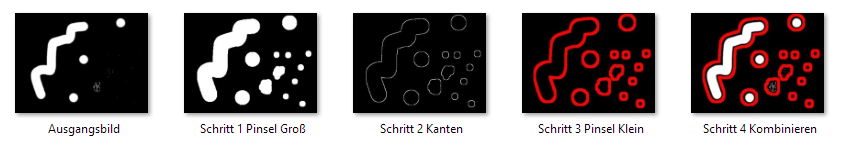
\includegraphics[scale=0.7]{images/L-mask.png}
		\caption{Selbst kleine Details sind gro� Umrandet und gut Sichtbar}
		\label{fig:L: Mask}
	\end{figure}
	
	\lstinputlisting{sources/ConvolveOpCircleItExample.java}
	
	
	
	
	
	\clearpage
	
	
%--------------------------------------------------------------------------
% Anhang
%--------------------------------------------------------------------------

  \phantomsection
  \addcontentsline{toc}{chapter}{Anhang}
	\addcontentsline{toc1}{section}{Abbildungsverzeichnis}
	\listoffigures
	\newpage
	\phantomsection
	
	\addcontentsline{toc}{section}{Tabellenverzeichnis}
	\listoftables
	\newpage
	\phantomsection

	\addcontentsline{toc}{section}{Verzeichnis der Listings}
	\lstlistoflistings
	\newpage
	\phantomsection
	
	%\addcontentsline{toc}{section}{Index}
  \printindex
  \newpage
  \phantomsection
  
	\addcontentsline{toc}{section}{Literaturverzeichnis}
	%\bibliographystyle{alpha} 		 %Standardstyle
	%\bibliographystyle{dinat}		 %Style und Layout nach DIN 1502
	%\bibliography{tiger}					 %Literaturverzeichnis einf�gen
	
	
	%So kann zitiert werden (sollte in einer der Unterdateien sein)
	%\citep[vgl. Seite 22]{kopka1:00}
	
	\begin{thebibliography}{999}
		



\bibitem[L: StegoGeschichte]{L: StegoGeschichte} 
\url{https://igw.tuwien.ac.at/designlehren/steganographie.pdf} \\
Eine kurze Geschichte der Steganographie \\ 
Peter Purgathofer \\
12.11.2016

\bibitem[L: Stego VS Crypto]{L: Stego VS Crypto}
\url{http://digilib.happy-security.de/files/Steganographie.pdf} \\
Kryptographie und Informationstheorie: Steganographie \\
Prof. Dr. Richard Eier, Institut f�r Computertechnik TU Wien\\
Michaela Schuster \ltodo{Ist Schuster der Autor oder Dr. Richard Eier? Au�erdem - Ist das so richtig als Quelle drinnen?}\\
20.11.2016 

\bibitem[L: StegoVersteck]{L: StegoVersteck}
\url{http://www.tecchannel.de/a/vertrauliche-daten-perfekt-versteckt,2024281} \\
Vertrauliche Daten perfekt versteckt, Artikel vom 30.11.2009 \\
pte pte\\
13.12.2016


\bibitem{L: USA-Crypto Export}
\url{https://en.wikipedia.org/wiki/Export_of_cryptography_from_the_United_States}

		
		\bibitem[Kopka1]{kopka1:00} 
		Helmut Kopka:
		  \emph{Latex Band 1, Einf�hrung} \\ 
		  Addison-Wesley, 2000  \\
		  ISBN: 3-8273-7038-8
		\bibitem[Demmig 1]{demig:04}
		  Demmig, Thomas: \\
			\emph{jetzt lerne ich Latex 2} \\
			Markt+Technik, 2004 \\
			ISBN 3-8272-6517-7
		\bibitem[Web 1]{Web:01}
		\href{http://www.meta-x.de/faq/LaTeX-Einfuehrung.html}{http://www.meta-x.de/faq/LaTeX-Einfuehrung.html}\\
		Latex-Einf"uhrung\\
		28.September 2012
		\bibitem[JavaDoc05]{JavaDoc:05}
		\href{http://docs.oracle.com/cd/E12839\_01/core.1111/e10043/introjps.htm}{http://docs.oracle.com/cd/E12839\_01/core.1111/e10043/introjps.htm}\\
		Oracle Security Guide �ber das Java Sicherheits Model\\
		13.11.2014
	\end{thebibliography} 
	\newpage
	\phantomsection
\end{document}